
\section{Experiments}
\noindent{\bf Implementation Details.} Consistent with previous works~\cite{tan2024harnessing,jiang2023cross}, we utilize the CLIP ViT-B/16 model as our backbone. Following IRRA~\cite{jiang2023cross}, we incorporate a randomly initialized multimodal interaction encoder to facilitate masked token prediction. 
Our implementation processes 384×128 resolution images with a maximum length of $N=77$ text sequences. We employ Adam~\cite{kingma2014adam} as the optimizer, initialized with a learning rate of $1e-4$ and a weight decay of $4e-5$. The parameters $\beta_1$ and $\beta_2$ are set to 0.9 and 0.999, respectively. The temperature parameter $\tau$ in SDM loss is set to 0.02. We train GA-DMS for 30 epochs with a batch size of 512 on 8 NVIDIA A100~(80G) GPUs. For generating synthetic templates and captions, we utilize Qwen2.5-72B-Instruct~\cite{yang2024qwen2}, Qwen2.5-VL-7B-Instruct, and Qwen2.5-VL-32B-Instruct~\cite{bai2025qwen2}. Additionally, vLLM~\cite{kwon2023efficient} is leveraged to accelerate large-scale inference. Please refer to the Appendix ~\ref{Appendix hyper} for more detailed hyperparameters.


\begin{table*}[t!]
\centering
\resizebox{\linewidth}{!}{
\renewcommand{\arraystretch}{1.2}
\begin{tabular}{l|cc|cccc|cccc|cccc}
\toprule[1pt]
\multirow{2}{*}{\textbf{Method}} & \multirow{2}{*}{\textbf{Image Enc.}} & \multirow{2}{*}{\textbf{Text Enc.}} & \multicolumn{4}{c|}{\textbf{CUHK-PEDES}} & \multicolumn{4}{c|}{\textbf{ICFG-PEDES}} & \multicolumn{4}{c}{\textbf{RSTPReid}}  \\ \cline{4-15} 
&  &  & \textbf{R1} & \textbf{R5} & \textbf{R10} & \textbf{mAP} & \textbf{R1} & \textbf{R5} & \textbf{R10} & \textbf{mAP} & \textbf{R1} & \textbf{R5} & \textbf{R10} & \textbf{mAP} \\ 
\midrule
% CMPM/C \cite{zhang2018deep} & RN50  &LSTM &49.37  & -  &79.27 & -  &43.51 &65.44 &74.26 & - & - & -  & -& - \\
ViTAA \cite{wang2020vitaa} &RN50 &LSTM &55.97 &75.84  &83.52 &- &50.98 & 68.79 & 75.78 & -& - & - & -  & -  \\
% DSSL \cite{zheng2020dual} & RN50 & BERT & 59.98  & 80.41  & 87.56 & - & -  & - & - & - & 32.43 & 55.08 & 63.19 & - \\ 
SSAN \cite{ding2021semantically} & RN50 & LSTM & 61.37 & 80.15 & 86.73 & - & 54.23 & 72.63 & 79.53 & - & 43.50 & 67.80 &77.15 & - \\ 
% LapsCore \cite{wu2021lapscore}& RN50 & BERT & 63.40  & -& 87.80 & -  & - & -& -  & -  & -  & -  & -  & -  \\
LBUL \cite{wang2022look}& RN50& BERT & 64.04  & 82.66  & 87.22 & - & -  & - & - & - & 45.55 & 68.2  & 77.85 & -  \\
% Han et al. \cite{han2021text} & CLIP-RN101 & CLIP-Xformer & 64.08 & 81.73 & 88.19 & 60.08 & - & - & - & - & - & - & - & - \\
SAF \cite{li2022learning} & ViT-Base  & BERT  & 64.13  & 82.62  & 88.4  & -  & - & -  & -  & -  & -  & -  & -  & -  \\
TIPCB \cite{chen2022tipcb} & RN50 & BERT & 64.26  & 83.19  & 89.1  & -     & 54.96  & 74.72 & 81.89 & -     & -     & -     & -     & -     \\
CAIBC \cite{wang2022caibc} & RN50 & BERT & 64.43  & 82.87  & 88.37 & -     & -   & -     & -     & -     & 47.35 & 69.55 & 79.00 & -     \\
AXM-Net \cite{farooq2022axm}  & RN50  & BERT & 64.44  & 80.52  & 86.77 & 58.70 & -  & -     & -     & -     & -     & -     & -     & -     \\
LGUR \cite{shao2022learning} & DeiT-Small  & BERT  & 65.25  & 83.12  & 89.00 & - & 59.02 & 75.32 & 81.56 & - & 47.95 & 71.85 & 80.25 & -     \\
IVT \cite{shu2022see} & ViT-Base  & BERT  & 65.69  & 85.93  & 91.15 & -  & 56.04   & 73.60 & 80.22 & -  & 46.70 & 70.00 & 78.80 & -     \\
LCR²S \cite{yan2023learning}  & RN50  & TextCNN+BERT  & 67.36  & 84.19  & 89.62 & 59.20 & 57.93  & 76.08 & 82.40 & 38.21 & 54.95 & 76.65 & 84.70 & 40.92 \\
UniPT \cite{shao2023unified}  & ViT-Base & BERT   & 68.50  & 84.67  & 90.38 & -  & 60.09  & 76.19 & 82.46 & -  & 51.85 & 74.85 & 82.85 & -     \\
\midrule

\multicolumn{6}{l}{\textit{with ALBEF \cite{li2021align} backbone:}} \\
\midrule
RaSa \cite{bai2023rasa}  & CLIP-ViT & BERT-base & 76.51  & 90.29  & 94.25 & 69.38 & 65.28  & 80.40  & 85.12 & 41.29 & 66.90 & 86.50 & 91.35 & 52.31 \\
APTM \cite{yang2023towards} & Swin-B & BERT-base & 76.53  & 90.04  & 94.15 & 66.91 & 68.51 & 82.99 & 87.56 & 41.22 & 67.50 & 85.70 & 91.45 & 52.56 \\ 
\midrule
\multicolumn{6}{l}{\textit{with CLIP \cite{radford2021learning} backbone:}} \\
\midrule
Han et al. \cite{han2021text} & CLIP-RN101 & CLIP-Xformer & 64.08 & 81.73 & 88.19 & 60.08 & - & - & - & - & - & - & - & - \\
IRRA \cite{jiang2023cross} & CLIP-ViT  & CLIP-Xformer & 73.38  & 89.93  & 93.71 & 66.10 & 63.46   & 80.25 & 85.82 & 38.06 & 60.20 & 81.30 & 88.20 & 47.17 \\

% \multicolumn{1}{l|}{MDRL \cite{yang2024multi}} & CLIP-ViT & \multicolumn{1}{c|}{CLIP-Xformer} &\multicolumn{1}{l}{74.56} & \multicolumn{1}{l}{92.56} & \multicolumn{1}{l}{96.30} & \multicolumn{1}{c|}{-} & 65.88 &85.25 &90.38  & \multicolumn{1}{c|}{-} & -  & -  & - & -  \\

\multicolumn{1}{l|}{FSRL \cite{wang2024fine}} & CLIP-ViT & \multicolumn{1}{c|}{CLIP-Xformer} & \multicolumn{1}{l}{74.65} & \multicolumn{1}{l}{89.77} & \multicolumn{1}{l}{94.03} & \multicolumn{1}{c|}{67.49} & 64.01 & 80.42 & 85.56 & \multicolumn{1}{c|}{39.64} & 60.20 & 81.40 & 88.60 & 47.38 \\

\multicolumn{1}{l|}{Propot \cite{yan2024prototypical}} & CLIP-ViT & \multicolumn{1}{c|}{CLIP-Xformer} & \multicolumn{1}{l}{74.89} & \multicolumn{1}{l}{89.90} & \multicolumn{1}{l}{94.17} & \multicolumn{1}{c|}{67.12} & 65.12 & 81.57 & 86.97 & \multicolumn{1}{c|}{\textbf{42.93}} & 61.87 & 83.63 & 89.70 & 47.82 \\

\multicolumn{1}{l|}{SAP-SAM \cite{wang2024fine}} & CLIP-ViT & \multicolumn{1}{c|}{CLIP-Xformer} & \multicolumn{1}{l}{75.05} & \multicolumn{1}{l}{89.93} & \multicolumn{1}{l}{93.73} & \multicolumn{1}{c|}{-} & 63.97 & 80.84 & 86.17 & \multicolumn{1}{c|}{-} & 62.85 & 82.65 & 89.85 & - \\

\multicolumn{1}{l|}{PLOT \cite{park2025plot}} & CLIP-ViT & \multicolumn{1}{c|}{CLIP-Xformer} & \multicolumn{1}{l}{75.28} & \multicolumn{1}{l}{90.42} & \multicolumn{1}{l}{94.12} & \multicolumn{1}{c|}{-} & 65.76 & 81.39 & 86.73 & \multicolumn{1}{c|}{-} & 61.80 & 82.85 & 89.45 & - \\

\multicolumn{1}{l|}{RDE \cite{qin2024noisy}} & CLIP-ViT & \multicolumn{1}{c|}{CLIP-Xformer} & \multicolumn{1}{l}{75.94} & \multicolumn{1}{l}{90.14} & \multicolumn{1}{l}{94.12} & \multicolumn{1}{l|}{67.56} & 67.68 & 82.47 & 87.36 & \multicolumn{1}{c|}{40.06} & 65.35 & 83.95 & 89.90 & 50.88 \\
% \hdashline
% MALS \cite{yang2023towards} + IRRA & CLIP-ViT & CLIP-Xformer &74.05  & 89.48 & 93.64 & 66.57  & 64.37  & 80.75   & 86.12   &38.85  &61.90  &80.60  &89.30  & 48.08 \\

% LUPerson-T \cite{shao2023unified} + IRRA  & CLIP-ViT  & CLIP-Xformer  & 74.37 &89.51 & 93.97 & 66.60 & 64.50  &80.24  & 85.74  &38.22  & 62.20 &83.30 & 89.75 &48.33  \\

% SYNTH-PEDES \cite{zuo2024plip}+ IRRA & CLIP-ViT & CLIP-Xformer & 74.25 & 89.49 & 93.68 & 66.52 & 65.79 & 81.94 & 87.32 & 39.43 & 64.35 & 83.75 & 91.00 & 50.93 \\

NAM \cite{tan2024harnessing} & CLIP-ViT & CLIP-Xformer & 76.82 & 91.16 & 94.46 & 69.55 & 67.05 & 82.16 & 87.33 & 41.51 & 68.50 & 87.15 & 92.10 & 53.02 \\

Ours (1.0 M) & CLIP-ViT  & CLIP-Xformer & \underline{77.02} &\underline{91.28} &\underline{94.58} &\underline{69.65} &\underline{69.07} &\underline{83.26} &\underline{87.64} &41.91 &\underline{70.30} &\underline{88.00} &\underline{92.85}&\underline{54.89} \\

Ours (5.0 M) & CLIP-ViT  & CLIP-Xformer & \textbf{77.60} &\textbf{91.40} &\textbf{94.78} &\textbf{69.82} &\textbf{69.51} &\textbf{83.47} &\textbf{87.67} &\underline{42.30} &\textbf{71.25} &\textbf{87.25} &\textbf{92.90} &\textbf{55.43} \\
\bottomrule
\end{tabular}}
\vspace{-2mm}
\caption{Comparisons with state-of-the-art methods in the traditional evaluation settings. The best results are marked in \textbf{bold}, and the
second-best results are \underline{underlined}.}
\label{tab:sota-traditional}
\vspace{-5mm}
\end{table*}

\noindent{\bf Evaluation.} Following previous works~\cite{tan2024harnessing, qin2024noisy}, we conduct a comprehensive evaluation of our method across three challenging text-to-image person retrieval datasets: CUHK-PEDES~\cite{li2017person}, ICFG-PEDES~\cite{ding2021semantically}, and RSTPReid~\cite{zhu2021dssl}. We employ Rank-$k$ ($k$=1, 5, 10) and mean Average Precision (mAP) as evaluation metrics for all datasets.

\begin{figure}[t!]
  \centerline{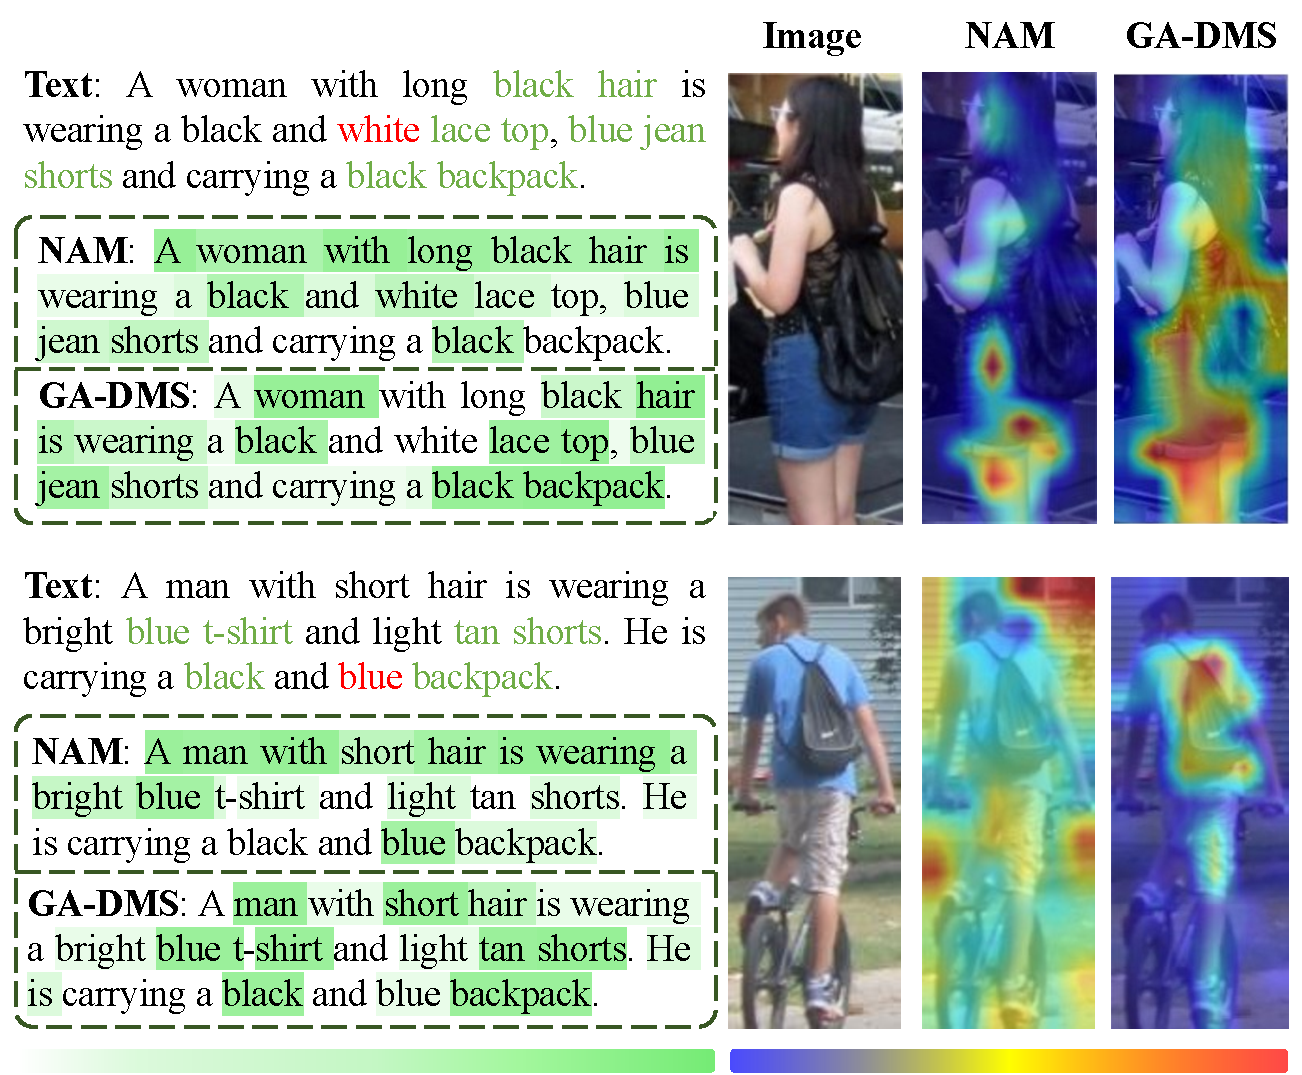
\includegraphics[width=\linewidth]{Figure/weight_visual3.pdf}}
  \vspace{-2mm}
  \caption{Visualization of token-wise weight scores and attention maps generated by NAM~\cite{tan2024harnessing} and our GA-DMS.}
  \label{fig-visual}
  \vspace{-5mm}
\end{figure}

\begin{table}[t]
\centering
\resizebox{0.49\textwidth}{!}{%
\renewcommand{\arraystretch}{1.2}
\begin{tabular}{l|cc|cc|cc}
    \toprule
    \multirow{2}{*}{\textbf{Pre-training Dataset}} & \multicolumn{2}{c|}{\textbf{CUHK-PEDES}} & \multicolumn{2}{c|}{\textbf{ICFG-PEDES}} & \multicolumn{2}{c}{\textbf{RSTPReid}} \\ \cline{2-7} 
    & \textbf{R1} & \textbf{mAP} & \textbf{R1} & \textbf{mAP} & \textbf{R1} & \textbf{mAP} \\ 
    \midrule 
    None & 12.65 & 11.15 & 6.67 & 2.51 & 13.45 & 10.31 \\
    MALS (1.5M) & 20.47 & 18.46 & 11.71 & 4.57 & 21.50 & 16.95 \\
    LUPerson-T (0.95M) & 21.55 & 18.76 & 11.20 & 4.53 & 22.15 & 17.29 \\ 
    SYNTH-PEDES (1.0M) & 57.29  & 51.86 &\textbf{57.13}  &\textbf{31.36} & 42.20 & 32.28 \\ 
    LUPerson-MLLM (1.0M) & 56.01  & 50.34 & 37.00 & 20.21  &50.60  &37.08 \\
    \midrule
    Ours (0.1 M) & 58.95  & 52.77  & 38.18  &19.70  &47.10   &36.68  \\
    Web-Person (1.0 M) & \underline{66.26} &\underline{58.54}  &51.99 &28.81 &\underline{55.35} &\underline{40.57} \\ 
    Ours (5.0 M) & \textbf{68.34} &\textbf{60.22}  &\underline{54.64} &\underline{30.68} &\textbf{57.60} &\textbf{42.00} \\ 
    \bottomrule
\end{tabular}
}
\vspace{-2mm}
\caption{Comparisons with existing pre-training datasets in the direct transfer setting. The best results are marked in \textbf{bold}, and the
second-best results are \underline{underlined}.}
\label{tab:zero-shot}
\vspace{-5mm}
\end{table}

\subsection{Comparison with Existing Methods.} 
We evaluate GA-DMS against state-of-the-art methods on three benchmarks: CUHK-PEDES, ICFG-PEDES, and RSTPReid. As shown in Tab.~\ref{tab:sota-traditional}, our pre-trained model achieves superior performance after fine-tuning with the IRRA~\cite{jiang2023cross}, which significantly improves Rank-1 accuracy and mAP on the RSTPReid dataset by 10.10\% and 7.72\% over the baseline of IRRA.  Compared with the NAM~\cite{tan2024harnessing}, GA-DMS obtains 0.2\%, 2.02\%, and 1.8\% improvement in Rank-1 on the CUHK-PEDES, ICFG-PEDES, and RSTPReid datasets, respectively. The primary reason for this improvement is that our proposed GA-DMS framework effectively distinguishes between noise and informative tokens based on the gradient-attention similarity score. As shown in Fig.~\ref{fig-visual}, compared with NAM~\cite{tan2024harnessing}, our GA-DMS can better allocate weights to text tokens while concentrating attention on human-centric regions. This capability not only reduces the effect of noise on model training but also improves the model’s capacity to learn fine-grained semantic information. Moreover, upon scaling the WebPerson dataset from 1.0 M to 5.0 M, GA-DMS achieves new state-of-the-art Rank-1 accuracies of 77.6\%, 69.51\%, and 71.25\% across three downstream datasets.


\begin{table}[t!]
\centering
\resizebox{0.49\textwidth}{!}{%
\renewcommand{\arraystretch}{1.2}
\begin{tabular}{l|c|clclcl}
\toprule[1pt]
\multirow{3}{*}{\textbf{Pre-training Dataset}} & \multirow{3}{*}{\textbf{Source}} & \multicolumn{6}{c}{\textbf{Target}} \\ \cline{3-8} 
 &  & \multicolumn{2}{c|}{\textbf{CUHK-PEDES}} & \multicolumn{2}{c|}{\textbf{ICFG-PEDES}} & \multicolumn{2}{c}{\textbf{RSTPReid}} \\ \cline{3-8} 
 &  & \textbf{R1} & \multicolumn{1}{l|}{\textbf{mAP}} & \textbf{R1} & \multicolumn{1}{l|}{\textbf{mAP}} & \textbf{R1} & \textbf{mAP} \\ 
\midrule

\multirow{3}{*}{None} & CUHK-PEDES & \cellcolor{gray!30}{73.48} & \multicolumn{1}{l|}{\cellcolor{gray!30}{66.21}} & 43.04 & \multicolumn{1}{l|}{22.45} & 52.55 & 39.97 \\
 & ICFG-PEDES & 33.90 & \multicolumn{1}{l|}{31.65} & \cellcolor{gray!30}{63.83} & \multicolumn{1}{l|}{\cellcolor{gray!30}{38.37}} & 47.45 & 36.83 \\
 & RSTPReid & 35.25 & \multicolumn{1}{l|}{32.35} & 33.58 & \multicolumn{1}{l|}{19.58} & \cellcolor{gray!30}{60.40} & \cellcolor{gray!30}{47.70} \\ 
\midrule
 
\multirow{3}{*}{MALS(1.5 M)} & CUHK-PEDES & \cellcolor{gray!30}{73.67} & \multicolumn{1}{l|}{\cellcolor{gray!30}{65.23}} & 46.02 & \multicolumn{1}{l|}{24.06} & 55.05 & 41.29 \\
 & ICFG-PEDES & 43.11 & \multicolumn{1}{l|}{38.93} & \cellcolor{gray!30}{65.21} & \multicolumn{1}{l|}{\cellcolor{gray!30}{38.52}} & 48.45 & 37.29 \\
 & RSTPReid & 44.51 & \multicolumn{1}{l|}{39.99} & 40.78 & \multicolumn{1}{l|}{25.42} & \cellcolor{gray!30}{64.05} & \cellcolor{gray!30}{50.08} \\ 
 \midrule
 
\multirow{3}{*}{LUPerson-T(0.95 M)} & CUHK-PEDES & \cellcolor{gray!30}{74.28} & \multicolumn{1}{l|}{\cellcolor{gray!30}{66.52}} & 44.83 & \multicolumn{1}{l|}{22.72} & 54.25 & 39.26 \\
 & ICFG-PEDES & 34.66 & \multicolumn{1}{l|}{32.51} & \cellcolor{gray!30}{65.33} & \multicolumn{1}{l|}{\cellcolor{gray!30}{38.45}} & 48.30 & 38.51 \\
 & RSTPReid & 39.26 & \multicolumn{1}{l|}{34.26} & 34.95 & \multicolumn{1}{l|}{22.25} & \cellcolor{gray!30}{61.50} & \cellcolor{gray!30}{48.28} \\ 
 \midrule

\multirow{3}{*}{SYNTH-PEDES(1.0 M)} & CUHK-PEDES & \cellcolor{gray!30}{74.12} & \multicolumn{1}{l|}{\cellcolor{gray!30}{65.82}} & 57.14 & \multicolumn{1}{l|}{32.12} & 55.85 & 40.85 \\
 & ICFG-PEDES & 60.49 & \multicolumn{1}{l|}{54.61} & \cellcolor{gray!30}{66.63} & \multicolumn{1}{l|}{\cellcolor{gray!30}{39.32}} & 49.80 & 37.34 \\
 & RSTPReid & 57.75 & \multicolumn{1}{l|}{53.01} & 53.88 & \multicolumn{1}{l|}{30.88} & \cellcolor{gray!30}{66.75} & \cellcolor{gray!30}{52.18} \\ 
\midrule
 
\multirow{3}{*}{LUPerson-MLLM(1.0 M)} & CUHK-PEDES & \cellcolor{gray!30}{76.59} & \multicolumn{1}{l|}{\cellcolor{gray!30}{68.06}} & 47.17 & \multicolumn{1}{l|}{25.41} & 59.35 & 43.76 \\
 & ICFG-PEDES & 60.75 & \multicolumn{1}{l|}{54.42} & \cellcolor{gray!30}{67.18} & \multicolumn{1}{l|}{\cellcolor{gray!30}{40.27}} &55.65 & 44.05 \\
 & RSTPReid & 60.04 & \multicolumn{1}{l|}{53.85} & 46.39 & \multicolumn{1}{l|}{27.91} & \cellcolor{gray!30}{69.45} & \cellcolor{gray!30}{53.30} \\ 
\midrule
 
\multirow{3}{*}{Ours(0.1 M)} & CUHK-PEDES & \cellcolor{gray!30}{75.53} & \multicolumn{1}{l|}{\cellcolor{gray!30}{67.92}} & 47.79 & \multicolumn{1}{l|}{25.14} & 56.75 & 41.01 \\

 & ICFG-PEDES & 58.67 & \multicolumn{1}{l|}{52.66} & \cellcolor{gray!30}{66.35} & \multicolumn{1}{l|}{\cellcolor{gray!30}{39.95}} & 52.93 & 39.84 \\

 & RSTPReid & 58.49 & \multicolumn{1}{l|}{52.50} & 44.41 & \multicolumn{1}{l|}{25.98} & \cellcolor{gray!30}{65.90} & \cellcolor{gray!30}{49.28} \\ 
 \midrule
 
\multirow{3}{*}{Ours(1.0 M)} & CUHK-PEDES & \cellcolor{gray!30}{\underline{77.02}} & \multicolumn{1}{l|}{\cellcolor{gray!30}{\underline{69.65}}} & \underline{57.24} & \multicolumn{1}{l|}{\underline{32.13}} & \underline{61.10} & \underline{45.27} \\
 & ICFG-PEDES & \underline{68.16} & \multicolumn{1}{l|}{\underline{60.79}} & \cellcolor{gray!30}{\underline{69.07}} & \multicolumn{1}{l|}{\cellcolor{gray!30}{\underline{41.91}}} &\underline{59.15} & \underline{44.94} \\
 & RSTPReid & \underline{68.41} & \multicolumn{1}{l|}{\underline{61.28}} & \underline{56.13} & \multicolumn{1}{l|}{\underline{34.64}} & \cellcolor{gray!30}{\underline{70.30}} & \cellcolor{gray!30}{\underline{54.89}} \\ 
\midrule

\multirow{3}{*}{Ours(5.0 M)} & CUHK-PEDES & \cellcolor{gray!30}{\textbf{77.60}} & \multicolumn{1}{l|}{\cellcolor{gray!30}{\textbf{69.82}}} & \textbf{58.91} & \multicolumn{1}{l|}{\textbf{33.70}} & \textbf{61.80} & \textbf{46.81} \\
 & ICFG-PEDES & \textbf{69.83} & \multicolumn{1}{l|}{\textbf{62.06}} & \cellcolor{gray!30}{\textbf{69.52}} & \multicolumn{1}{l|}{\cellcolor{gray!30}{\textbf{42.30}}} &\textbf{60.05} & \textbf{45.46} \\
 & RSTPReid & \textbf{69.19} & \multicolumn{1}{l|}{\textbf{62.00}} & \textbf{57.13} & \multicolumn{1}{l|}{\textbf{35.76}} & \cellcolor{gray!30}{\textbf{71.25}} & \cellcolor{gray!30}{\textbf{55.43}} \\ 
 \bottomrule
\end{tabular}
}
\vspace{-2mm}
\caption{Comparisons with existing pre-training datasets in the fine-tuning setting. The best results are marked in \textbf{bold}, and the second-best results are \underline{underlined}. \colorbox{gray!30}{Gray} indicates that the source and target are homologous.}
\label{tab:sota-finetune}
\vspace{-5mm}
\end{table}

\subsection{Comparison with Existing Datasets.} We conduct comprehensive comparisons between our WebPerson dataset and four existing large-scale pre-training datasets: MALS~\cite{yang2023towards}, LUPerson-T~\cite{shao2023unified}, SYNTH-PEDES~\cite{zuo2024plip}, and LUPerson-MLLM~\cite{tan2024harnessing}. MALS consists of 1.5 million synthetic images generated using commercial diffusion models, with textual descriptions automatically produced by BLIP~\cite{li2022blip}. LUPerson-T includes 0.95 million images, each enhanced by one of 456 templates to maximize caption diversity. SYNTH-PEDES provides 4.8 million images, each annotated with an average of 2.53 textual descriptions, generated through a hybrid architecture that combines a ResNet101-FPN~\cite{he2016deep} visual encoder with a GPT-2~\cite{radford2019language} text generator for detailed person attribute modeling. Notably, LUPerson-MLLM utilizes two multimodal large language models for caption generation, supplemented by 46 ChatGPT-optimized templates obtained through iterative dialogues to enhance linguistic variation. This dataset comprises 1.0 million images, each paired with two MLLM-generated captions. 


Tab.~\ref{tab:zero-shot} presents comparative results under a direct transfer setting, where models pre-trained on Web-Person exhibit superior cross-dataset generalization across three benchmarks. Specifically, under the comparable 1M dataset, our constructed WebPerson dataset demonstrates superior performance on CUHK-PEDES and RSTPReid, and shows suboptimal performance on ICFG-PEDES. Notably, the WebPerson dataset demonstrates comparable performance to the full-scale LUPerson-MLLM even when trained on a mere 0.1M samples. These experimental results demonstrate that our proposed WebPerson dataset exhibits strong robustness and can learn person representations with enhanced transferability.


As shown in Tab.~\ref{tab:sota-finetune}, we also evaluate the fine-tuning performance following LUPerson-MLLM~\cite{tan2024harnessing}, utilizing the IRRA with models pretrained on different datasets. Results indicate that WebPerson pretraining yields state-of-the-art performance across both in-domain and cross-domain scenarios. At the 1M data scale, WebPerson achieves consistent improvements over LUPerson-MLLM, with Rank-1 accuracy gains of 0.43\%, 1.89\%, and 0.85\% on CUHK-PEDES, ICFG-PEDES, and RSTPReid respectively. The cross-domain evaluations reveal particularly significant performance enhancements, highlighting WebPerson's exceptional representation transferability through fine-tuning.


\subsection{Ablation Study}

\begin{table}[t!]

\centering
\setlength{\tabcolsep}{4pt} % 缩小列间距
\resizebox{0.49\textwidth}{!}{%
\renewcommand{\arraystretch}{1.2}
\begin{tabular}{cc|cc|cc|cc|cc}
\toprule
\multicolumn{2}{c|}{\textbf{Masking Method}} & \multicolumn{2}{c|}{\textbf{Components}} & \multicolumn{2}{c|}{\textbf{CUHK-PEDES}} & \multicolumn{2}{c|}{\textbf{ICFG-PEDES}} & \multicolumn{2}{c}{\textbf{RSTPReid}} \\
\midrule
\textbf{CSS} & \textbf{GASS} & \textbf{SDM} & \textbf{MTP} & \textbf{R1} & \textbf{mAP} & \textbf{R1} & \textbf{mAP} & \textbf{R1} & \textbf{mAP} \\
\midrule
\xmark &\xmark &\xmark &\xmark  & 56.75 & 50.42 & 34.63 & 17.59 & 45.50 & 34.51 \\
\midrule
\checkmark & \xmark &\xmark & \checkmark & 56.35 & 50.21 & 34.72 & 17.66 & 44.60 & 33.28 \\
\checkmark &\xmark & \checkmark &\xmark & 63.29 & 57.42 & 43.39 & 24.12 & 51.95 & 39.41 \\
\checkmark &\xmark & \checkmark & \checkmark & 62.74 & 57.01 & 42.96 & 23.88 & 50.80 & 38.91 \\
\midrule
\xmark &\checkmark &\xmark & \checkmark& 57.29 & 52.28 & 36.24 & 18.96 & 47.90 & 35.97 \\
\xmark &\checkmark & \checkmark &\xmark & \underline{63.87} & \underline{57.56} & \underline{44.02} & \underline{24.18} & \underline{52.30} & \underline{39.61} \\
\xmark &\checkmark & \checkmark & \checkmark & \textbf{64.25} & \textbf{58.27} & \textbf{44.39} & \textbf{24.67} & \textbf{52.70} & \textbf{40.12} \\
\bottomrule
\end{tabular}
}
\vspace{-2mm}
\caption{Ablation on different components and masking methods. CSS: Cosine Similarity Score. GASS: Gradient-Attention Similarity Score. SDM: Similarity Distribution Matching. MTP: Masked Token Prediction.}
\label{tab:ablation_components}
\vspace{-5mm}
\end{table}
\noindent{\bf Ablation on Different Components and Masking Methods.}
To substantiate the efficacy of various components and the effectiveness of our proposed Gradient-Attention Similarity Score~(GASS), we perform a comprehensive ablation study with a 0.5M data sample from our WebPerson dataset. As shown in Tab.~\ref{tab:ablation_components}, the integrating Masked Token Prediction (MTP) with GASS improves performance across all evaluation metrics, as predicting semantically rich tokens enhances fine-grained learning. The Similarity Distribution Matching (SDM) component alone enhances image-text alignment by replacing noisy tokens with learnable embeddings, achieving Rank-1 accuracy gains of 7.12\%, 9.39\%, and 6.8\% on CUHK-PEDES, ICFG-PEDES, and RSTPReid respectively. By combining MTP with SDM, we observe enhancements across all metrics, further substantiating the efficacy of the components within our method.

When comparing Cosine Similarity Score (CSS) with Gradient-Attention Similarity Score (GASS), GASS consistently exhibits superior performance. This advantage primarily stems from GASS's capacity to precisely weight textual tokens during training by incorporating gradient and attention information. As illustrated in Fig.~\ref{fig-visual}, our method accurately allocates weights to noise textual tokens (\textit{e.g.}, "white lace top"), thereby effectively mitigating the influence of noise on the model's representation learning.

\begin{figure}[t!]
\begin{subfigure}[b]{\linewidth}
\centering
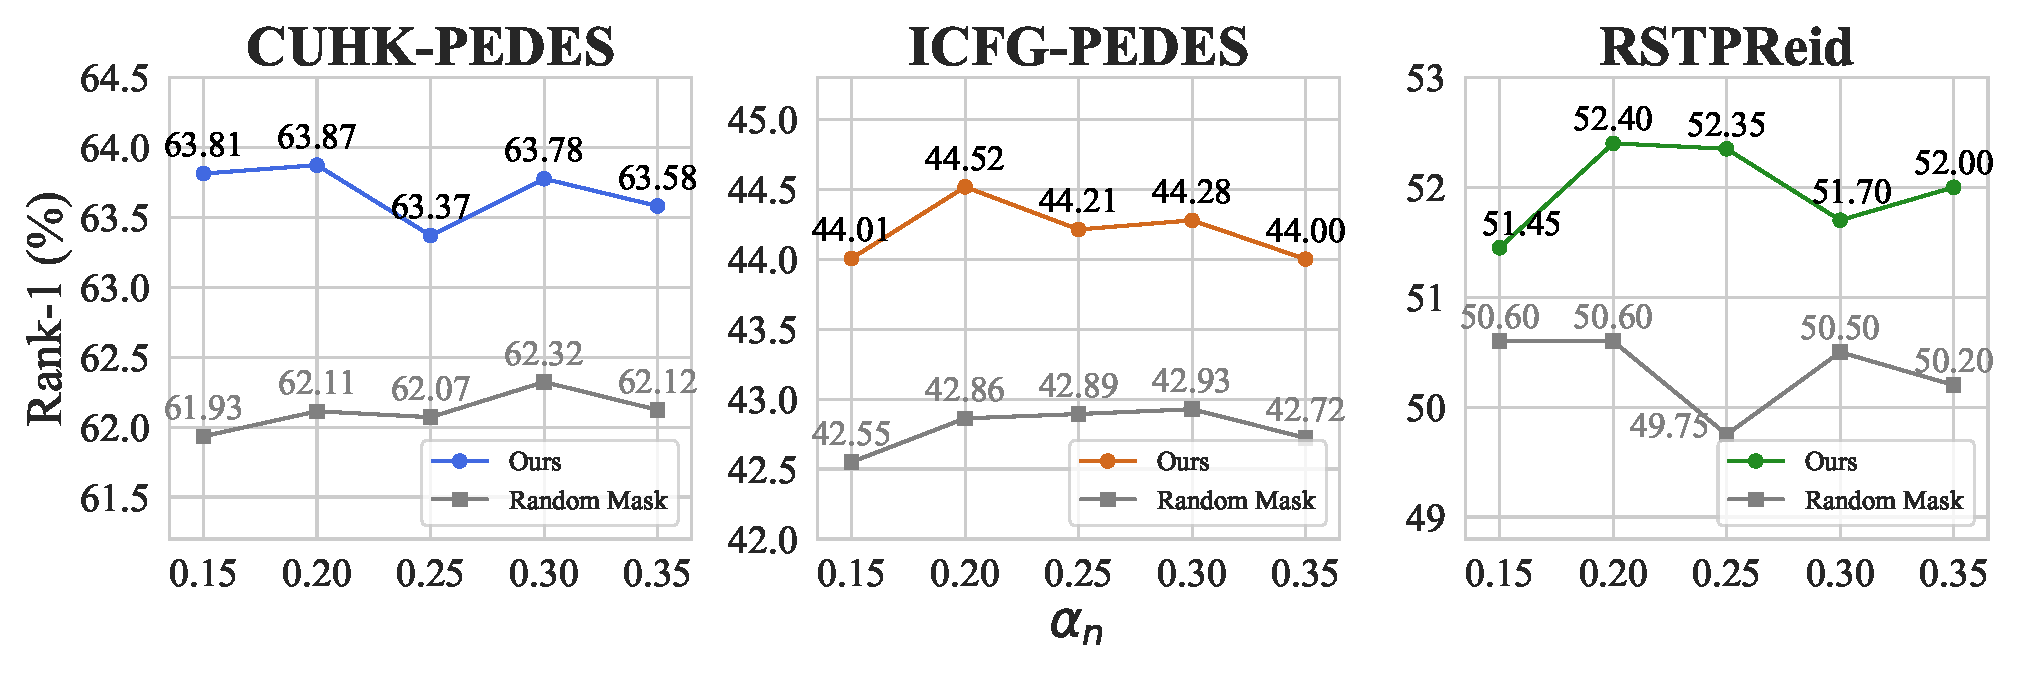
\includegraphics[width=1.0\linewidth]{Figure/NTM.pdf}
\vspace{-7mm}
\subcaption{\small Ablation on $\alpha_{n}$ for masking noise tokens}
\label{fig:NAM}
\end{subfigure}
\hfill
\begin{subfigure}[b]{\linewidth}
\centering
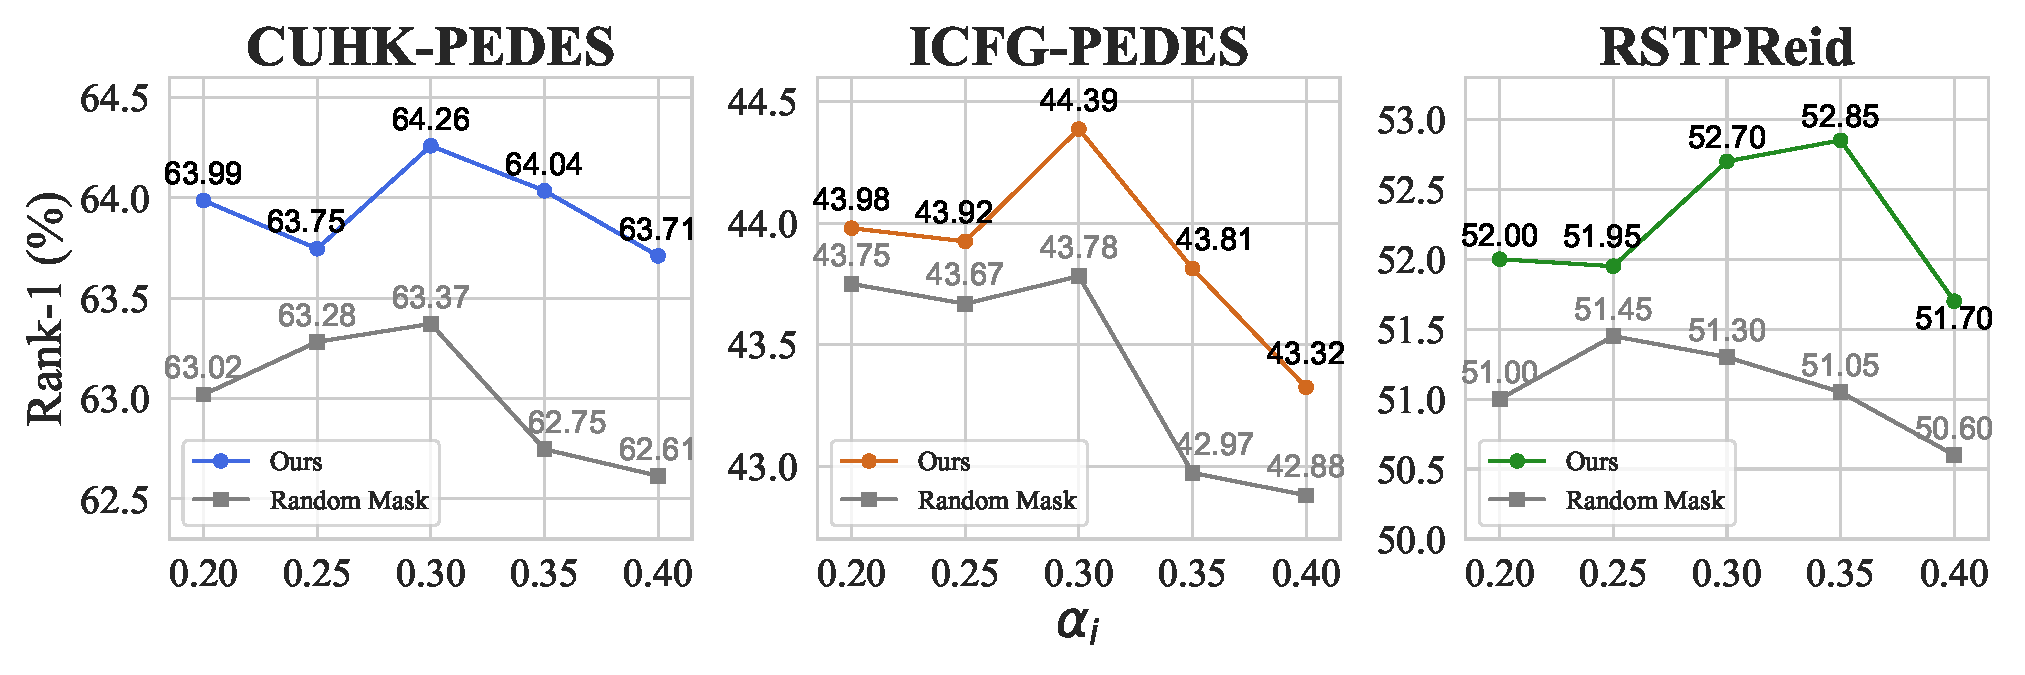
\includegraphics[width=1.0\linewidth]{Figure/MTP.pdf}
\vspace{-7mm}
\subcaption{\small Ablation on $\alpha_{i}$ for masking informative tokens}
\label{fig:MLM}
\end{subfigure}
\vspace{-7mm}
\caption{Ablation experiment results for $\alpha_{n}$ and $\alpha_{i}$, which can directly influence the upper limit of the masking probability for noise and informative tokens.}
\vspace{-3mm}
\label{fig:Ratio}
\end{figure}


\noindent{\bf Ablation on \textbf{$\alpha_{n}$} and \textbf{$\alpha_{i}$}.} 
In this work, our dual-masking synergetic learning method dynamically masks textual tokens according to gradient-attention similarity scores. We introduce parameters $\alpha_{n}$ and $\alpha_{i}$ to regulate the maximum masking probabilities for noise and informative tokens. Fig.~\ref{fig:Ratio} presents an ablation study on $\alpha_{n}$ and $\alpha_{i}$ to determine the optimal settings. For enhanced performance on three downstream datasets, we set $\alpha_{n}=0.2$ and $\alpha_{i}=0.3$. Additionally, our method consistently outperforms random masking baselines, confirming its effectiveness.

\begin{figure}[t]
% \setlength{\abovecaptionskip}{0pt}
  \centerline{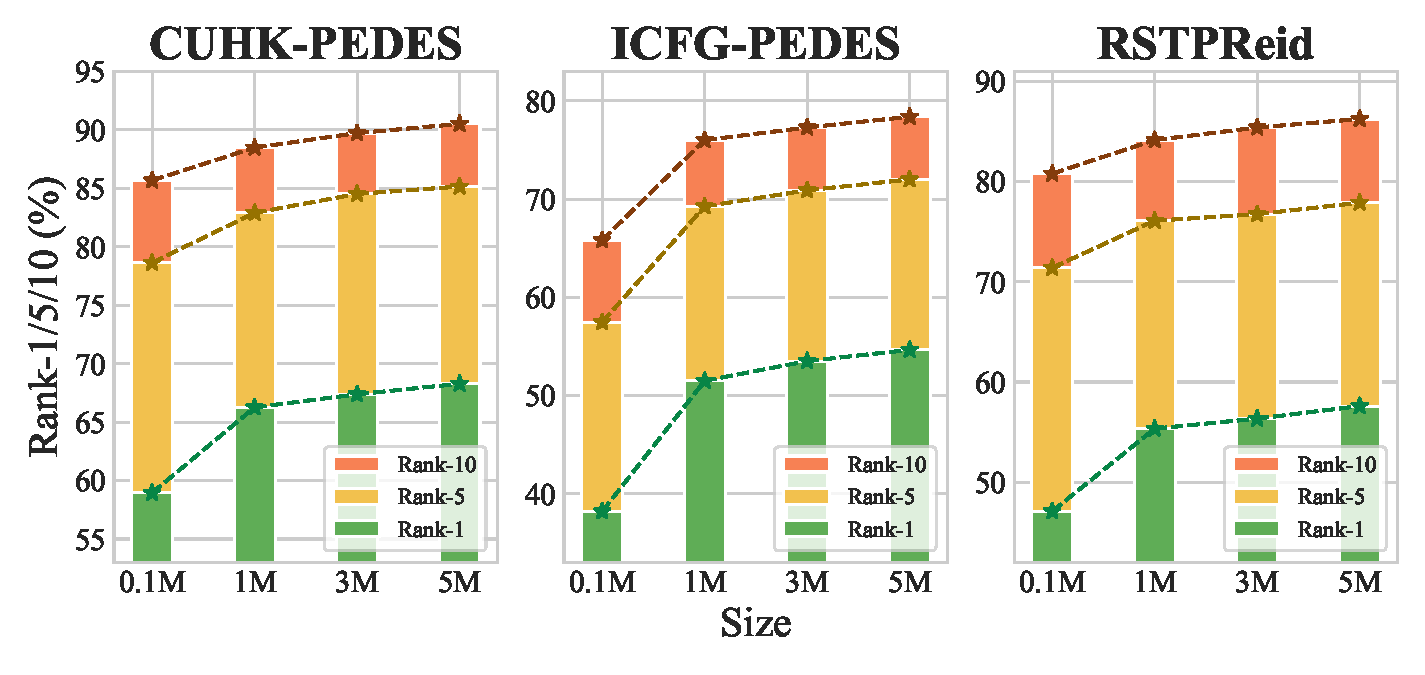
\includegraphics[width=1.0\linewidth]{Figure/SIZE.pdf}}
  \vspace{-5mm}
  \caption{Data scaling analysis of WebPerson dataset.The performance of our GA-DMS method in direct transfer settings.}
  \label{fig:size}
  \vspace{-5mm}
  % \vspace{-0.5em}
\end{figure}

\noindent{\bf Data Scaling Analysis.}
%分析数据量对性能的影响：
To explore the impact of pretraining data scale on person representation learning, we systematically augmented the dataset size from 0.1M to 1M, 3M, and 5M samples for pertaining. Fig.~\ref{fig:size} illustrates the direct transfer performance evaluation across three benchmarks at different data scales. The outcomes consistently reveal performance enhancements as the data volume increases. At the maximum scale of 5.0M samples, the model demonstrates Rank-1 accuracy improvements of 9.39\%, 16.46\%, and 10.50\% across the three benchmarks in comparison to the 0.1M baseline, indicating a clear upward trajectory. These findings conclusively demonstrate that scaling high-quality pretraining data substantially enhances text-based person retrieval capability.

